%% ============================================================================
%% DRAFT -- ReMoto, new version -- manuscript for the Journal of Computational
%% Neuroscience (Springer). Not submitted; not for the public repository yet.
%%
%% Class: Springer Nature LaTeX template (sn-jnl.cls), APA reference style, two
%% columns ("iicol"), as the journal's submission guidelines ask (read on
%% 2026-11-22). The class is NOT in this folder: open the "Springer Nature LaTeX
%% Template" on Overleaf and upload this file, references.bib and figures/.
%% This file has not been compiled yet (no TeX on the machine where it was
%% written): expect to fix small things on the first run.
%%
%% Before submission the journal asks for NO subfolders: move figures/Fig*.pdf
%% next to this file and delete the \graphicspath line.
%%
%% Everything only the authors can fill in is marked "TODO(authors)" in a
%% comment and, where text is missing, shows in red in the PDF.
%% ============================================================================

\documentclass[pdflatex,sn-apa,iicol]{sn-jnl}

\usepackage{graphicx}
\usepackage{multirow}
\usepackage{amsmath,amssymb,amsfonts}
\usepackage{amsthm}
\usepackage{mathrsfs}
\usepackage[title]{appendix}
\usepackage{xcolor}
\usepackage{textcomp}
\usepackage{manyfoot}
\usepackage{booktabs}
\usepackage{url}

\graphicspath{{figures/}}

\newcommand{\TODO}[1]{\textcolor{red}{[TODO: #1]}}
\providecommand{\code}[1]{\texttt{#1}}
\providecommand{\dd}{\mathrm{d}}

\raggedbottom

\begin{document}

% TODO(authors): choose the final title and the version name ("3.0" is the version
% of the Maven artifacts, 3.0.0-SNAPSHOT; it is not used in the text below).
\title[ReMoto: a reproducible reimplementation]{ReMoto revisited: porting a Web-based simulator of spinal motor nuclei to a reproducible platform with bit-for-bit verification}

% TODO(authors): complete the author list, order, ORCIDs, affiliations and the
% corresponding author's e-mail. Only the first author is known from the repository;
% nothing below about affiliation was assumed.
\author*[1]{\fnm{Rogerio R. L.} \sur{Cisi}}\email{to-be-completed@example.org}

\affil*[1]{\orgdiv{TODO: department}, \orgname{TODO: institution}, \orgaddress{\city{TODO: city}, \country{TODO: country}}}

% Word count of the abstract: 245 (the journal asks for 150 to 250, with no undefined
% abbreviations and no references).
\abstract{ReMoto is a simulator of the spinal cord circuits that control the human ankle muscles, with conductance-based motoneurons and interneurons, afferent fibers, descending tracts, muscles, electromyogram, proprioceptors and joint mechanics. It was introduced in this journal in 2008 as a Web application, but its software stack no longer receives security updates, part of its interface no longer runs in current browsers, and it drew random numbers without a seed, so no simulation could be repeated. A new version keeps the published models and replaces everything around them: a numerical core without dependencies, scenarios stored as files, a Web application without accounts, a command-line runner and a seeded random source. The models were ported in slices, requiring every output to stay identical, bit for bit, to that of the original code, checked through hashes of reference outputs for the thirty configurations of the original database. Results are also identical for any number of threads, because neurons are updated in parallel only where no random number is drawn and every synaptic delay exceeds one integration step. The work exposed two defects in the inherited code. Since 2016, synaptic conductances had not decayed between events, which raised the simulated soleus force by 47\% in the default scenario; and the order of gamma-distributed descending commands was never stored, which silenced them. The first is corrected under an engine version recorded with every run; the order is now saved with the scenario. The simulator and twenty scenarios are freely available.}

\keywords{Neuromuscular simulation, Motoneuron pool, Spinal cord, Reproducibility, Research software, Legacy code}

\maketitle

%% ============================================================================
\section{Introduction}\label{sec:intro}
%% ============================================================================

ReMoto is a simulator of the spinal cord circuits that control muscles, built to interpret human neurophysiological experiments, to test hypotheses about neuronal dynamics and to teach neurophysiology \citep{Cisi2008}. It represents the motor nuclei of four ankle muscles (soleus, medial and lateral gastrocnemius, tibialis anterior) with two-compartment motoneurons of types S, FR and FF, Renshaw cells and other spinal interneurons, Ia, II and Ib afferents, descending tracts modeled as stochastic point processes, and electrical stimulation of nerves with orthodromic and antidromic propagation. Each motoneuron spike produces, after a conduction delay, a motor-unit action potential and a twitch, and their sums give the electromyogram (EMG) and the muscle force. Later work added active dendrites with persistent inward currents \citep{Elias2012,Elias2013}, studied how the statistics of the descending command shape force and EMG variability \citep{Watanabe2013}, closed the loop with proprioceptors and an inverted-pendulum model of upright stance \citep{Elias2014}, and showed that fast oscillatory commands from the motor cortex can be decoded by the spinal cord for force control \citep{Watanabe2015}.

The simulator has also been used to study the depression of the H-reflex \citep{Cisi2007}, force fluctuations in a motoneuron pool \citep{Kohn2009}, the effect of activation-dependent muscle stiffness on proprioceptive feedback and the short-latency reflex \citep{Chaud2012}, the H and T reflexes \citep{Mezzarane2013}, the low-frequency fluctuations of plantar-flexion torque in force and position tasks \citep{Watanabe2013ner}, the identification of a motor-unit pool \citep{Watanabe2014} and the effect of neurodegenerative diseases on sensorimotor control \citep{Elias2018,Oliveira2022}, and in the teaching of neuroscience \citep{EliasKohn2013teaching}.
% TODO(authors): the project site lists nine more conference presentations, without DOIs;
% they are transcribed at the end of references.bib for you to add if you want them cited.

General-purpose simulators such as NEURON \citep{Hines1997}, NEST \citep{Gewaltig2007}, Brian~2 \citep{Stimberg2019} and NetPyNE \citep{DuraBernal2019} cover the neuronal part of such a system, and musculoskeletal packages such as OpenSim \citep{Delp2007} cover the mechanical part. Models of the motor-unit pool with force and EMG generation \citep{Fuglevand1993,Dideriksen2010} sit between the two. ReMoto was designed for the whole chain from descending command to joint torque in one tool, configured through a Web page, so that an experimentalist can set up a virtual version of an H-reflex or force-control experiment without programming. A version of ReMoto written in Fortran, announced on the project site, was later adapted to study Guillain--Barr\'e syndrome \citep{Oliveira2022}.
% TODO(authors): describe the relation between the Java code base of this paper and the
% Fortran versions announced on the project site on 2024-06-26
% (github.com/rnwatanabe/projectFR and github.com/oliveiramarina/ReMoto_AIDP). They were
% not examined for this draft; in particular, whether the 2016 change to the synapses
% (Section 3.3) has a counterpart there is not known.

That Web page is what aged. The original system was a Java Web application built on Struts~1 and JavaServer Pages, served by Apache Tomcat~7, with an HSQLDB database for users and configurations and Java applets for part of the interface. Struts~1 and Tomcat~7 no longer receive security updates, and applets are not run by any current browser. The original site is still served at the time of writing.
% TODO(authors): state the present status of the original site. On 2026-11-23 its landing
% page (remoto.leb.usp.br, "Current Version: 2.1"), its News page and the Quick Guide of
% the application (main.do) opened in a browser; logging in, running a simulation and the
% applets were not tried.
The code also called \code{Math.random()} and \code{new Random()} without a seed, so two runs of the same configuration never gave the same spike trains and no published figure could be regenerated exactly. Reproducibility of simulation results is a long-standing concern in computational neuroscience \citep{Crook2013,McDougal2016,Eglen2017}, and reproducing a model from its original code can be hard even when that code is available \citep{Pauli2018,Rougier2017}.

This paper describes a new version of ReMoto, 3.0, that keeps the published models and replaces the platform around them. The last release of the Web application was 2.1, in December 2011, preceded by 2.0 (July 2011) and 1.1.5 (2008).
% TODO(authors): the release dates above come from the Downloads page of the project site,
% read on 2026-11-23, which also lists a 2.2 beta (June 2012) and a standalone 2.0 for
% Windows. Confirm them, and confirm that the new version should be numbered 3.0 (it is
% 3.0.0-SNAPSHOT in the Maven modules).
We set one requirement for the port: the new code had to give the same numbers as the old one, bit for bit, in every output, and every exception had to be deliberate, tested and recorded. This is stricter than the statistical comparison used when a model is moved between simulators \citep{Gutzen2018,Trensch2018}, and it was possible here because the language stayed the same. It turned the original program into the specification of the new one, in the way characterization tests are used on legacy software \citep{Feathers2004}. The requirement had a scientific return as well: holding the outputs fixed while the code was taken apart exposed two defects in the inherited code, one of which had changed the dynamics of every synapse since 2016.

The contributions are (i) a description of the new architecture, in which a simulation is fully determined by a scenario file, a seed and an engine version; (ii) the method used to port a legacy simulator with bit-for-bit equivalence, including the behavior of the database that the old code relied on without stating it; (iii) a parallel update of the neurons whose results do not depend on the number of threads; and (iv) the analysis of the two defects and of their effect on the simulated motor output.

%% ============================================================================
\section{Methods}\label{sec:methods}
%% ============================================================================

\subsection{Models kept from the original simulator}\label{sec:models}

The models are those of the original publications, and only the elements needed to follow the rest of the paper are summarized here. Parameter values and their sources are given by \citet{Cisi2008}, \citet{Elias2012}, \citet{Elias2013}, \citet{Watanabe2013} and \citet{Elias2014}.

\subsubsection{Neurons and synapses}\label{sec:neurons}

A motoneuron has a somatic and a dendritic compartment with membrane potentials $V_s$ and $V_d$, measured from rest ($E_0 = 0$) and limited to the interval from $-16$ to $120$\,mV:
\begin{align}
C_d \frac{\dd V_d}{\dd t} &= g_c (V_s - V_d) + g_{Ld} (E_0 - V_d) \nonumber\\
 &\quad + \gamma_{Ca}\, g_{Ca}(t)\,(E_{Ca} - V_d) + I_{\mathrm{syn},d} + I_{\mathrm{inj},d}, \label{eq:dend}\\
C_s \frac{\dd V_s}{\dd t} &= g_c (V_d - V_s) + g_{Ls} (E_0 - V_s) \nonumber\\
 &\quad + \sum_{x} g_x(t)\,(E_x - V_s) + I_{\mathrm{syn},s} + I_{\mathrm{inj},s}, \label{eq:soma}
\end{align}
where $C$ are capacitances, $g_L$ leak conductances, $g_c$ the coupling conductance, $I_{\mathrm{inj}}$ injected currents, and $x$ runs over the sodium ($g_{Na} = \bar g_{Na} m^3 h$), fast potassium ($\bar g_{Kf} n^4$) and slow potassium ($\bar g_{Ks} q^2$) channels. The dendritic calcium conductance ($\bar g_{Ca}\, p$) carries the persistent inward current and is scaled by $\gamma_{Ca}$, which is zero for a passive dendrite \citep{Elias2012}. Gating variables follow first-order kinetics whose rate constants switch for a pulse of fixed duration when the soma crosses its threshold outside the refractory period, in the manner of the pulse-based models of \citet{Destexhe1997}.
% TODO(authors): confirm that Destexhe (1997) is the source the original paper gives for the
% pulse-based channels; the reference itself was checked, the attribution was not.
Interneurons have the somatic compartment only.

Each compartment has one group of excitatory and one group of inhibitory synapses, with current $I_{\mathrm{syn}} = G(t)\,(E_{\mathrm{syn}} - V)$. A presynaptic spike arrives after the delay of its synapse and releases transmitter for a pulse of fixed duration, during which the bound fraction $r$ of that synapse follows the kinetic scheme of \citet{Destexhe1994},
\begin{equation}
\frac{\dd r}{\dd t} = \alpha\, T(t)\,(1 - r) - \beta\, r , \label{eq:kinetics}
\end{equation}
with $T = T_{\max}$ during the pulse and $T = 0$ otherwise, so that $r$ rises towards $r_\infty = \alpha T_{\max} / (\alpha T_{\max} + \beta)$ with time constant $\tau_{\mathrm{on}} = 1 / (\alpha T_{\max} + \beta)$ and then decays with $\tau_{\mathrm{off}} = 1/\beta$. Instead of integrating one equation per synapse, the group keeps two sums in the way proposed by \citet{Lytton1996}: $R_{\mathrm{on}}$ over the synapses in a pulse and $R_{\mathrm{off}}$ over the others, each with a closed-form solution since the time $t_0$ of the last event (the start or the end of any pulse in the group),
\begin{align}
R_{\mathrm{on}}(t) &= N_{\mathrm{on}} r_\infty \nonumber\\
 &\quad + \bigl[ R_{\mathrm{on}}(t_0) - N_{\mathrm{on}} r_\infty \bigr] e^{-(t - t_0)/\tau_{\mathrm{on}}}, \label{eq:ron}\\
R_{\mathrm{off}}(t) &= R_{\mathrm{off}}(t_0)\, e^{-(t - t_0)/\tau_{\mathrm{off}}}, \label{eq:roff}\\
G(t) &= \bar G\, \bigl[ R_{\mathrm{on}}(t) + R_{\mathrm{off}}(t) \bigr], \label{eq:gsyn}
\end{align}
where $\bar G = \sum_i \bar g_i$ is the sum of the maximal conductances of the group, each synapse enters with weight $\bar g_i / \bar G$, and $N_{\mathrm{on}}$ is the sum of the weights of the synapses in a pulse. The stored values $R_{\mathrm{on}}(t_0)$, $R_{\mathrm{off}}(t_0)$ and $N_{\mathrm{on}}$ change only at events. A synapse may also show depression or facilitation, in which its maximal conductance is changed by a fixed percentage at each spike and recovers exponentially.

\subsubsection{Descending drive, afferents and stimulation}\label{sec:drive}

Descending tracts and independent noise sources are populations of axons that fire as point processes: Poisson, gamma of integer order, or Gaussian intervals. The mean interval (or the mean rate) can be modulated by a signal (constant, sine, amplitude-modulated sine, square, ramp, triangle, trapezoid, random and others). The gamma process integrates the rate until it reaches a threshold drawn as
\begin{equation}
\theta = -\frac{1}{k} \ln \prod_{i=1}^{k} U_i , \label{eq:gamma}
\end{equation}
with $U_i$ uniform in $[0, 1)$ and $k$ the order. Gaussian variates are approximated by the sum of twelve uniform variates, as in the original code. Afferent fibers (Ia, II, Ib) fire through a gamma process driven by the receptor output and can be activated by nerve stimulation; injected currents and nerve stimuli use the same family of modulating signals.

\subsubsection{Muscles, proprioceptors and joint}\label{sec:periphery}

% TODO(authors): add and cite the sources of the models below that are named in code
% comments but whose references were not checked for this draft (see the end of
% references.bib): Crago et al. (1982), Prochazka (1999), Raikova and Aladjov (2002),
% Hermite-Rodriguez MUAPs (Lo Conte et al.; Hermens et al., 1992), Arnold et al. (2010).
Each motor unit contributes a twitch and a motor-unit action potential. Muscle force is produced by one of three working models: a second-order critically damped system per unit, a Hill-type muscle with a tendon, or a twitch model named after Raikova in the code. The raw EMG is the sum of the motor-unit potentials, and the EMG shown by default adds noise and a band-pass filter from 50 to 1000\,Hz. The muscle spindle follows \citet{Mileusnic2006}, with a lumped alternative, and a lumped Golgi tendon organ model gives the Ib rate. The ankle is either isometric, an inverted pendulum \citep{Elias2014}, or a position task against a load.

\subsubsection{Numerical integration}\label{sec:integration}

Time advances with a fixed step $h$ (0.05\,ms in all public scenarios). In each step the nerves are updated first, then every neuron, then the musculotendon units and the joint. A motoneuron integrates Eq.~\eqref{eq:dend} with a fourth-order Runge-Kutta step using the somatic potential of the previous step, and then Eq.~\eqref{eq:soma} with the updated dendritic potential. The four Runge-Kutta stages ask the synaptic groups and the channels for their conductances at $t$, $t + h/2$ (twice) and $t + h$. Start and end of transmitter pulses are detected in those calls, with a tolerance of $10^{-3}$\,ms.

\subsection{Software architecture}\label{sec:architecture}

Version 3.0 is written in Java~25 and built with Maven as four modules (Fig.~\ref{fig:architecture}). Table~\ref{tab:stack} compares it with the original system.

\begin{figure*}[t]
\centering
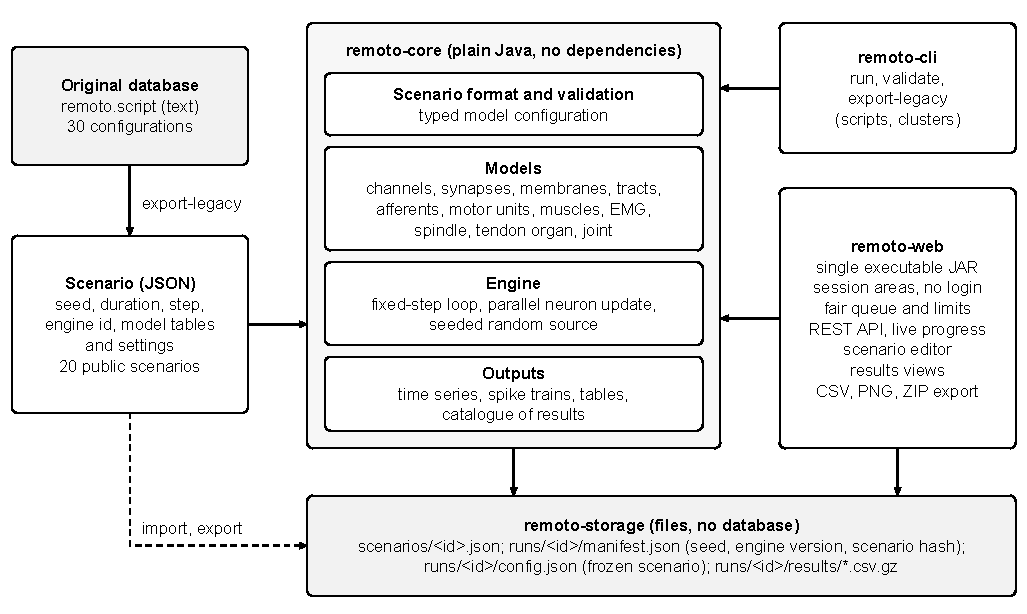
\includegraphics[width=\textwidth]{Fig1}
\caption{Architecture of the new version. A scenario file holds everything that defines a simulation. The core library turns it into the model, runs it and emits named outputs; the command-line runner and the Web application are two front ends over the same core, and both store scenarios and runs as plain files. Configurations of the original database are converted into scenarios by \code{export-legacy}, which reads the database file as text}\label{fig:architecture}
\end{figure*}

\begin{table*}[t]
\caption{The original system and the new version}\label{tab:stack}
\begin{tabular}{@{}p{0.17\textwidth}p{0.36\textwidth}p{0.40\textwidth}@{}}
\toprule
 & Original system & New version \\
\midrule
Language and runtime & Java 8, Apache Tomcat 7 & Java 25, one executable JAR with an embedded server \\
Web framework & Struts 1, JavaServer Pages, Java applets & Spring Boot 4, server-rendered pages with htmx and uPlot \\
Persistence & HSQLDB database (users, configurations) & Files: JSON scenarios and manifests, compressed CSV results \\
Users & Local accounts & No accounts: one private area per browser \\
Random numbers & \code{Math.random()}, \code{new Random()}, no seed & One seeded source per simulation thread \\
Parallelism & One thread per simulation & Neurons updated by several threads, same results \\
Use without the site & Ad hoc Java programs in the source tree & Command-line runner, REST interface \\
Provenance of a run & None & Scenario copy and hash, seed, engine version \\
Automated checks & Ad hoc scripts & Unit tests per model, reference hashes, continuous integration \\
\botrule
\end{tabular}
\end{table*}

\subsubsection{Core library and scenario format}\label{sec:core}

The core (\code{remoto-core}, 135 source files and about 20\,000 lines) is plain Java with no dependency outside the standard library. It contains the scenario format and its validation, the models, the engine and the conversion of old configurations. The models live in one package per family (ion channels, synapses, membranes, tracts, afferent fibers, stimuli, motor units and muscles, EMG, receptors, joints) and do not know about configuration or storage; a second layer assembles the network from the configuration and runs the loop of Section~\ref{sec:integration}.

A scenario is a JSON document with a name, a description, a seed, the simulated duration, the integration step, the identifier of the engine and the model configuration:

\begingroup\footnotesize
\begin{verbatim}
{ "name": "Default - Soleus contraction",
  "schemaVersion": 1,
  "seed": 17,
  "durationMs": 5000,
  "stepMs": 0.05,
  "engine": "legacy",
  "legacy": {
    "format": "remoto-legacy-db/1",
    "idConfiguration": 17,
    "tables":   { ... },
    "settings": { ... } } }
\end{verbatim}
\endgroup

\noindent The field \code{tables} holds the rows of each table of the original database for that configuration, without the table of users. The optional field \code{settings} holds the choices that the old editor offered but the old database never stored (Section~\ref{sec:editor}). Keeping the tables as they were, instead of designing a new parameter format, is what made exact equivalence testable: the same rows go through the same mapping as before. The engine identifier leaves room for future engines that read the same scenario; at present there is one, named \code{legacy} because it runs the original models.

The engine writes its results through a narrow interface with three kinds of output (time series, spike trains and tables) and a catalogue that describes each one. Besides muscle force, motoneuron spikes, joint torque and EMG, a run stores what the results page of the old site could show: muscle, tendon, spindle, tendon-organ and joint signals, the spike trains of every group, the membrane potentials and conductances of selected neurons, and tables with the properties of neurons and motor units.

\subsubsection{File storage and run provenance}\label{sec:storage}

There is no database. A scenario is one JSON file; a run is a folder with a manifest (status, seed, engine version, SHA-256 hash of the scenario, timestamps), a frozen copy of the scenario that was actually simulated, and one compressed CSV file per output. The guarantees a database used to give are provided as follows: files are written to a temporary name and renamed, so a reader never sees a partial file; one lock per user area serializes writers, while different areas write in parallel; an edit carries the hash of the version it started from and is refused if the file changed meanwhile; and when the server starts, runs that were queued or running are marked as interrupted.

The scenario, its seed and the engine version together determine every output bit for bit (Section~\ref{sec:checks}), so the manifest and the frozen scenario are a complete recipe for repeating a run.

\subsubsection{Web application}\label{sec:web}

The Web application is a single executable file with an embedded server, installed as an operating-system service; it needs only a Java runtime and a folder to write in. There are no accounts. Each browser gets a private area identified by a random identifier kept in a cookie, and that area holds copies of scenarios, edited scenarios and runs. The site stores no personal data. To keep work for longer or to move it elsewhere, users export scenarios as JSON files and runs as archives with the manifest, the scenario and every result as CSV, and import them again later; a scenario exported from the site is the same file that the command-line runner executes.

% TODO(authors): the limits below are the defaults documented in docs/nova-versao.md on
% 2026-11-22 (area kept by a 30-day cookie; at most 2 running and 20 queued runs per
% area, 20 per network address, 200 in the whole queue). The site was still changing on
% that day: confirm them, or drop the numbers, before submission.
Simulations are CPU-bound and can take minutes, so several users must be able to submit them without blocking one another. The server runs a fixed number of simulations at a time and keeps one queue per area, served in rotation, so that a batch submitted from one area does not delay a single run from another. Because areas are free to create, there are also limits per area (by default 2 running and 20 queued runs), per network address and for the whole queue. Progress is reported live, results are shown in interactive charts, and every action of the pages is available through a REST interface.

The scenario editor and the results page were rebuilt after those of the original site, with the same menus, screens, labels, units and limits, so that users of the old site and the descriptions in earlier publications remain valid.

\subsubsection{Command-line runner}\label{sec:cli}

The same core is available without a server. The command \code{remoto run} executes a scenario file and writes the run folder described above, with options for the duration, the seed and the number of threads; \code{remoto validate} checks scenario files; and \code{remoto export-legacy} converts configurations of the original database into scenarios. This is the intended route for scripted studies and for clusters.

\subsection{Seeded random numbers}\label{sec:rng}

All random draws of the models go through one class that holds a pseudo-random generator per thread. The engine seeds the generator of the simulation thread with the seed of the scenario before the network is built and clears it afterwards; code that used to call \code{new Random()} now obtains a generator derived from the current sequence. The generator is \code{java.util.Random}, which also backed \code{Math.random()} in the original code, so the distributions drawn by the models are unchanged and only their starting point became controllable. The noise added to the displayed EMG, which the old site drew in its charting layer, is now drawn by the engine from a generator seeded from the scenario.

Because the outputs depend on the order of the draws, that order is part of what must be preserved, both by the port (Section~\ref{sec:port}) and by the parallel update (Section~\ref{sec:parallel}).

\subsection{Porting with bit-for-bit equivalence}\label{sec:port}

\subsubsection{Reference outputs}\label{sec:golden}

The first step was to run the original numerical code, unchanged except for the seeded random source, inside the new platform, and to record SHA-256 hashes of its outputs. These hashes are the reference against which every later change was judged. They cover the three public scenarios of the old site (configurations 17, 24 and 42 of the database) in three groups (force, spikes and torque; EMG; all outputs including those of the results page) and all thirty configurations of the original database, each simulated for 40\,ms with its identifier as seed. The references for the thirty configurations were generated while the configuration was still read from the HSQLDB database by the original data-access code.

A hash comparison is deliberately unforgiving. Floating-point addition is not associative \citep{Goldberg1991}, so reordering a sum, replacing a division by a multiplication or changing the order in which two neurons are created changes the last bits of some output, and with them the hash. A failed comparison therefore meant one of two things: an unintended change, which was reverted, or an intended one, which was recorded in the engine version (Section~\ref{sec:version}).

\subsubsection{Reproducing the behavior of the database}\label{sec:hsqldb}

The original code read its parameters from the database through SQL queries, and the database took part in the numerical result in two ways that the code did not state. First, numeric columns were declared as \code{NUMERIC(128,4)}, so every parameter written by the old editor had been rounded to four decimal places, with ties rounded down, and decimal values stored in integer columns had been truncated. Second, the rows returned by a query with \code{ORDER BY} came in the order produced by the sorting algorithm of the database, which is not stable: rows with equal keys, such as the tracts of one nucleus, come out in an order that depends on the algorithm. That order fixes the order in which neurons are created, and so the order of the random draws.

To run without the database, the reader of the scenario tables reproduces both behaviors: the rounding and truncation rules, the handling of null values, and the row order of each query, using the same sorting procedure as HSQLDB 2.7.3 (quicksort with median of three and insertion sort for short ranges). The conversion tool reads the text file in which HSQLDB stores its data and needs no database engine either. A test checks that this export reproduces the published scenario files, and the thirty reference hashes generated through the real database guard the whole path.

\subsubsection{Replacing the original code in slices}\label{sec:slices}

The models were not rewritten in parallel with the old code and compared at the end. Each family of models was moved into the core and the running engine was switched to it at once, so that every step could be checked against the reference hashes, the comparison between one and four threads, and one simulated second of the three legacy scenarios. The order was: typed configuration without the database; ion channels and synapses; random draws, twitch and EMG filter; neuronal membranes; modulating signals and tract spike generators; injected current and nerve stimulation; afferent fibers, motor units, muscles, proprioceptors and joints; and finally the simulation loop and the assembly of the network. Models that the three legacy scenarios do not exercise were compared through variants of the default scenario that switch them on.

Before the original code was removed, the following were verified to be identical, bit for bit, to its outputs: one simulated second of the three legacy scenarios, 100\,ms of the thirty configurations of the database, and eighteen variants of the default scenario covering the muscle, joint and spindle models, the motor-unit distributions, nerve stimulation, injected current, and the signals and interval distributions of the tracts. The comparisons that needed the original code or the database were then replaced by reference hashes generated with them.

Equivalence was kept even where the original code is questionable, and each such place was documented instead of silently changed. Examples are the Hill-type muscle, which evaluates four Runge-Kutta stages but advances with an Euler step; a fourth muscle model, which never computed a force; and tests of the refractory period that are written differently for motoneurons and interneurons and are not equivalent in floating point. Section~\ref{sec:deviations} lists the places where the new version does differ.

\subsubsection{Editor equivalence}\label{sec:editor}

The scenario editor loads a scenario into the same configuration objects as the original site, presents the same fields with the same limits, and writes the tables back as the original data-access code wrote them, with the column types, rounding and row order of the original schema. Tests check that loading and saving without editing returns the same tables and the same simulation, and that editing every screen writes what the original code wrote to a real database, for the three legacy scenarios.

Some screens of the old editor changed properties that the old database never stored: the choice of joint, muscle, spindle and tendon-organ models, the distribution of motor units, joint angles, spindle gains and others. They were valid only during a browser session. They are now saved in the \code{settings} field of the scenario and applied after the tables are read; scenarios converted from the database have no such field and use the defaults of the original code.

\subsection{Parallel update of the neurons}\label{sec:parallel}

Profiling showed that most of the time went to the synaptic conductances, which are evaluated four times per step for each of the four groups of every motoneuron, to look-ups by text key repeated at every spike, and to the muscle force. Three kinds of change were made, each verified against the reference hashes: keys and target conductances are resolved once instead of at every spike; a synaptic group returns its previous value when asked twice for the same instant with no event in between, as two of the Runge-Kutta stages do; and the neurons of one step are updated by several threads.

The parallel update (Fig.~\ref{fig:parallel}) is required to give exactly the result of the serial loop, not a statistically similar one. Three properties make the two orders equivalent.

\begin{figure*}[t]
\centering
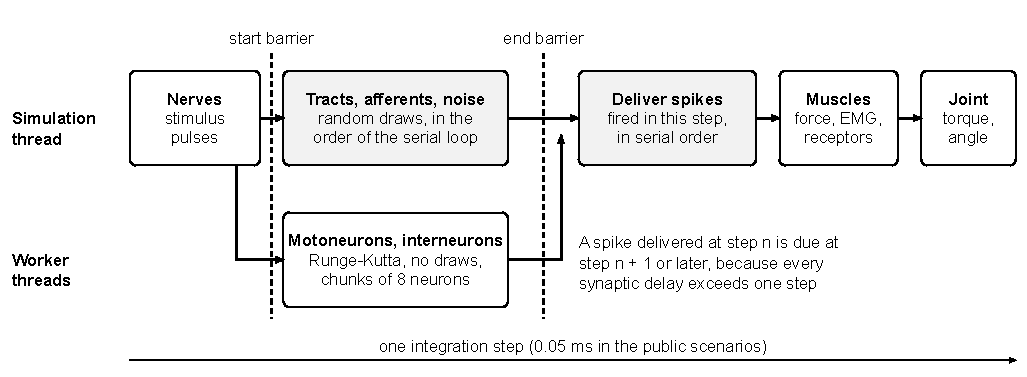
\includegraphics[width=\textwidth]{Fig2}
\caption{One integration step with the parallel update. Elements that draw random numbers run on the simulation thread in the order of the serial loop; motoneurons and interneurons, which draw none, are distributed over the threads in chunks. The spikes fired during the step are held by their neurons and delivered when all neurons have been updated, in the order in which the serial loop would have delivered them}\label{fig:parallel}
\end{figure*}

\emph{Spikes wait for the end of the step.} In the serial loop, a spike fired by neuron $j$ at step $n$ is queued at once at its targets with due time $t_n + d$, where $d$ is the synaptic delay, and a target updated later in the same step could see it. A synaptic group consumes a queued spike when it is asked for a time $t > t_n + d - \varepsilon$, with $\varepsilon$ the event tolerance, and during step $n$ it is asked for times up to $t_n + h$. If every delay satisfies
\begin{equation}
d \ge h + \varepsilon , \label{eq:delay}
\end{equation}
no spike fired during step $n$ can be consumed before step $n+1$, whatever the position of its source in the loop. Holding the spikes until all neurons are updated is then invisible to the dynamics, provided that they are delivered in the order of the serial loop, because each group consumes its queue in arrival order. The engine checks condition~\eqref{eq:delay} for every synapse when a simulation starts and falls back to the serial loop if it fails. The same idea, that the smallest delay bounds the interval over which neurons can be advanced independently, underlies distributed simulation in NEST and NEURON \citep{Morrison2005,Hines2008}.

\emph{Random draws stay on the simulation thread.} Only motoneurons and interneurons whose injected current is not modulated by a signal are updated in parallel; they draw no random numbers. Tracts, noise sources, afferent fibers and neurons with a modulated current are updated on the simulation thread in the order of the serial loop, so the sequence of draws does not change. The worker threads are given a generator that fails on use: a draw on a worker stops the simulation with an error instead of silently altering the results.

\emph{No shared writes.} A neuron updates only its own state and its own synaptic groups; the nerve, the injected current and global parameters are only read during the update.

The muscles, the proprioceptors and the joint are still updated on the simulation thread after the neurons. If fewer than 64 neurons qualify for parallel update, the serial loop is used.

\subsection{Engine version}\label{sec:version}

Every run records the version of the engine that produced it. The current identifier, \code{remoto-legacy-\allowbreak 2b5-\allowbreak rng1-\allowbreak syn1}, reads as the original code base (called 2b5), the first revision of the random source and the first revision of the synaptic conductances (Section~\ref{sec:synapse}). The rule is that outputs of the same scenario and seed are identical within one engine version and are not expected to be comparable across versions; any change that alters an output must change the version and regenerate the reference hashes in the same commit, with the reason stated.

\subsection{Simulations reported here}\label{sec:sims}

% TODO(authors): the simulations below were run for this draft on 2026-11-22 with the
% command-line runner built from the working tree of that day (HEAD f855a62 plus later
% commits that do not touch remoto-core). Re-run them on the tagged release that the
% paper will cite, archive the outputs and the plotting scripts, and update the numbers
% if anything changed. The plotting scripts, the hashes of the 49 outputs of each run and
% the commands are in paper/scripts (see its README), outside version control like the
% rest of paper/.
The simulations of Section~\ref{sec:results} used the command-line runner on a laptop with an Intel Core i5-10210U processor (four cores, eight hardware threads) and 20\,GB of memory, under Windows~11 and the Java HotSpot 64-bit virtual machine, version 25.0.2. The default scenario (configuration 17, seed 17, step 0.05\,ms) was run for its full 5\,s with four threads, and for 200\,ms and 1\,s with one, two and four threads for the checks of Section~\ref{sec:checks}. Outputs were compared through SHA-256 hashes of the decompressed CSV files. Firing rates were computed for motoneurons with at least two spikes between 1 and 5\,s as the number of intervals divided by the time between first and last spike in that window; force statistics refer to the same window.

To measure the effect of the 2016 change to the synaptic conductances (Section~\ref{sec:synapse}), a copy of the current sources was compiled in which the elapsed time $t - t_0$ of Eqs.~\eqref{eq:ron} and \eqref{eq:roff} can be replaced by the integration step through a runtime switch, with no other difference. With the switch off, this build gave outputs identical to those of the unmodified build.
% TODO(authors): this switch is not in the repository. It is the patch
% paper/scripts/synapse-2016-switch.patch (a system property read in SynapseGroup);
% decide whether to add it to the repository, for instance as a test-only option, so
% that readers can reproduce Fig. 4b and Table 3.
The single-synapse curves of Section~\ref{sec:synapse} were computed with a transcription of the arithmetic of the synaptic group for one synapse, called four times per step as a neuron calls it.

\subsection{Use of generative AI tools}\label{sec:ai}

% TODO(authors): the journal requires the use of large language models to be documented
% in the Methods. Facts available when this draft was written, for you to confirm and
% word as you see fit:
%  - 37 of the commits made to the repository from 2026-11-19 to 2026-11-22 carry the
%    trailer "Co-Authored-By: Claude Opus 5.5" (an AI coding assistant by Anthropic);
%  - this draft (text, figures and the simulations of Section 2.7) was produced on
%    2026-11-22 by Claude Code (model Claude Fable 5.2, Anthropic) from the repository
%    documentation, code and tests, at the request of the first author.
% The paragraph below is a proposal and must be made true before submission.
\TODO{authors to confirm and complete} The port of the simulator was carried out with the assistance of an AI coding assistant (Claude, Anthropic), as recorded in the commit history of the repository. Its changes were accepted only when the automated checks described in Section~\ref{sec:port} passed. A first draft of this manuscript was generated with the same kind of tool from the documentation, code and tests of the repository and from the simulations of Section~\ref{sec:sims}; the authors revised it and are responsible for its content.

%% ============================================================================
\section{Results}\label{sec:results}
%% ============================================================================

\subsection{Equivalence and repeatability}\label{sec:checks}

The automated test suite is part of the build and runs on a continuous-integration service at every push (Ubuntu with the Eclipse Temurin distribution of Java~25). Table~\ref{tab:tests} lists the tests that carry the equivalence claims of this paper.

\begin{table*}[t]
\caption{Automated tests that guard equivalence with the original code and repeatability}\label{tab:tests}
\begin{tabular}{@{}p{0.23\textwidth}p{0.72\textwidth}@{}}
\toprule
Test & What it guarantees \\
\midrule
Reference hashes & Outputs of configurations 17, 24 and 42 (40\,ms) match the hashes of force, spikes and torque, of the EMG, and of all outputs \\
Database configurations & Outputs of the thirty configurations of the original database (40\,ms, seed equal to the identifier) match hashes generated while the configuration was read from HSQLDB by the original code \\
Export without the database & Reading the database file as text reproduces the published scenario files, apart from descriptions and the documented changes of Section~\ref{sec:gamma} \\
Repeatability & The same seed gives identical outputs; a different seed gives different outputs \\
One and four threads & Configurations 17, 24 and 42 give identical outputs with one and with four threads; a worker thread cannot draw random numbers \\
Synapse and closed form & A synapse driven as by the Runge-Kutta integrator follows the closed-form solution: it rises during the pulse and decays after it \\
Editor and original code & Saving without editing preserves tables and simulation; editing every screen writes the tables that the original data-access code wrote to a real database \\
Complete model & A scenario with every model element switched on produces the outputs of each element \\
\botrule
\end{tabular}
\end{table*}

For this paper we made three further checks outside the test suite, on longer runs of the default scenario and on all 49 output files that a run of that scenario produces. (i) A run of 200\,ms with four threads and a run with one thread, made with two separately compiled copies of the program, gave identical files. (ii) Runs of 1\,s with four and with two threads gave identical files. (iii) The somatic spike trains and the muscle force of the 1-s run were identical to the first second of the 5-s run, so a shorter run is a prefix of a longer one for these outputs. The output of motoneuron spikes at the axon terminal of the 1-s run has 3266 spikes, the number recorded in the repository when the synaptic correction was made, before the models were moved to the core; the port did not change it.

The reference hashes stored in the repository were reproduced on two platforms: the laptop of Section~\ref{sec:sims} (Windows~11, Oracle's distribution of Java 25.0.2), where the tests of the core were run for this purpose, and the continuous-integration service (Ubuntu, Eclipse Temurin).
% TODO(authors): the CI runs seen for this draft were those of 22 and 23 November 2026, all
% successful. State on which system the hashes in golden-master.properties were first
% generated if that matters to the argument.

\subsection{Example: the default scenario}\label{sec:example}

The default scenario drives the soleus motor nucleus (900 motoneurons: 800 of type S, 50 FR and 50 FF) with 100 descending axons that fire as independent Poisson processes with a mean interval of 3\,ms, under isometric conditions. Figure~\ref{fig:default} shows outputs at four levels of the model. In the 5\,s simulated, 332 motoneurons were recruited, all of type S and most of them among the lowest indices of the pool (the highest was 553), along which the properties of the motoneurons are graded; they fired 16\,458 spikes. The 313 units with at least two spikes after the first second fired at $10.6 \pm 4.8$\,Hz (mean $\pm$ SD across units). Muscle force settled at $308.0 \pm 5.7$\,N (mean $\pm$ SD over time between 1 and 5\,s; coefficient of variation 1.9\%), with a plantar-flexion torque of 12.7\,N\,m in magnitude.

\begin{figure*}[t]
\centering
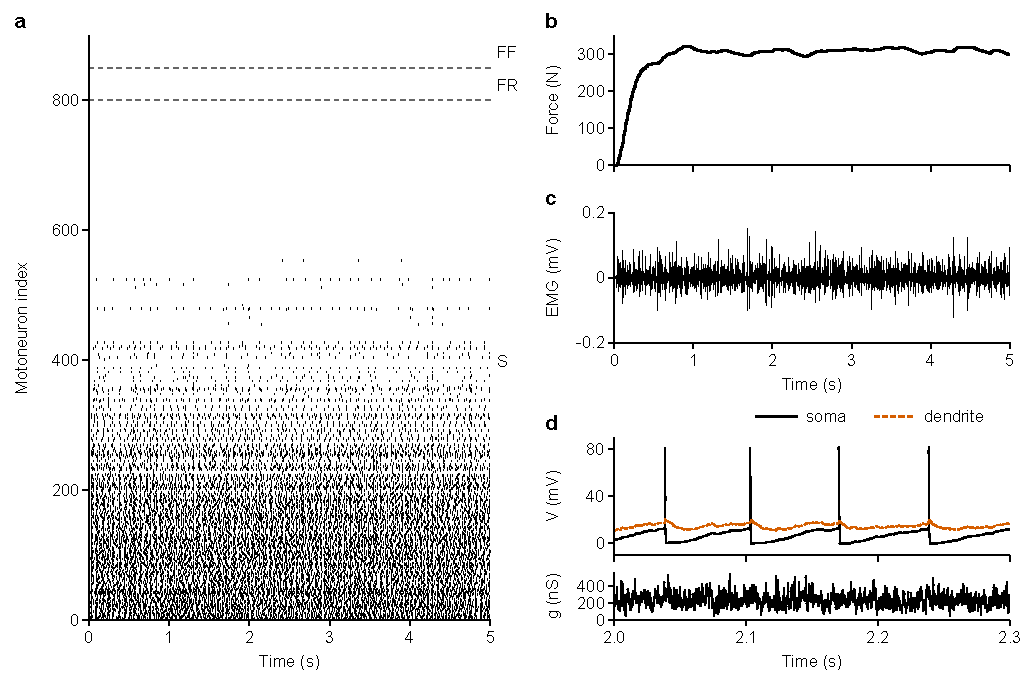
\includegraphics[width=\textwidth]{Fig3}
\caption{The default scenario (soleus nucleus driven by 100 descending axons, seed 17), 5\,s simulated. \textbf{a} Spikes of the 900 motoneurons at the axon terminal; dashed lines separate types S (indices 1 to 800), FR (801 to 850) and FF (851 to 900). \textbf{b} Soleus force. \textbf{c} Soleus EMG with noise and band-pass filter from 50 to 1000\,Hz. \textbf{d} Membrane potential of the first S-type motoneuron at the soma (solid line) and at the dendrite (dashed line), relative to rest, and below it the excitatory synaptic conductance of its dendrite, between 2.0 and 2.3\,s}\label{fig:default}
\end{figure*}

\subsection{First defect: synaptic conductances that did not decay}\label{sec:synapse}

In December 2016 a change to the parent repository replaced the elapsed time $t - t_0$ in Eqs.~\eqref{eq:ron} and \eqref{eq:roff} by the integration step $h$. Since $R_{\mathrm{on}}(t_0)$, $R_{\mathrm{off}}(t_0)$ and $N_{\mathrm{on}}$ are updated only when a pulse starts or ends, the right-hand sides then no longer depend on $t$: between two events of a group the conductance is constant. Figure~\ref{fig:synapse}a shows the consequence for one synapse and one presynaptic spike, with the parameters of the unit test ($\alpha = 1.1$\,mM$^{-1}$\,ms$^{-1}$, $\beta = 0.19$\,ms$^{-1}$, $T_{\max} = 1$\,mM, pulse of 1\,ms, $h = 0.05$\,ms). With the closed form the bound fraction rises to 0.618 at the end of the pulse and decays with $\tau_{\mathrm{off}} = 5.3$\,ms. With the 2016 code it steps to 0.053 during the pulse, then to 0.083, which is 13\% of the correct peak, and stays there until the next event in the same group, however far away that is. A synapse therefore delivered a smaller but unending conductance. In a group with many synapses the sums changed only at events, by one integration step of decay per event, so the time course of the conductance depended on the rate of events in the group and not on the time constants alone.

\begin{figure*}[t]
\centering
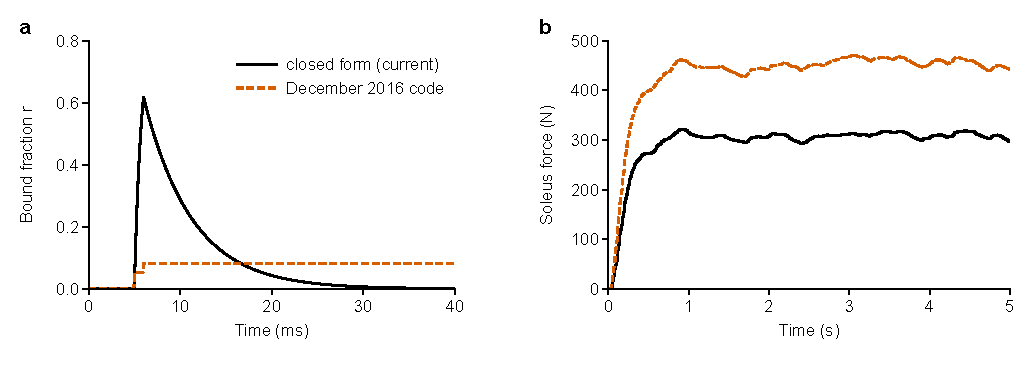
\includegraphics[width=\textwidth]{Fig4}
\caption{Effect of the 2016 change to the synaptic conductances. \textbf{a} Bound fraction of one synapse after one presynaptic spike at 5\,ms, computed with the closed form of Eqs.~\eqref{eq:ron} and \eqref{eq:roff} (solid line) and with the integration step in place of the elapsed time, as in the code from December 2016 (dashed line). \textbf{b} Soleus force in the default scenario with the current engine (solid line) and with the 2016 behavior switched back on (dashed line), for the same scenario and seed}\label{fig:synapse}
\end{figure*}

The engine returns to the closed form, which was the code in use until 2016. A unit test now compares the conductance of a synapse, called four times per step as the integrator calls it, with the analytical solution of Eq.~\eqref{eq:kinetics}, and requires it to fall below 1\% of its peak five time constants after the pulse.

To see what the defect did to the motor output, the default scenario was run with the 2016 behavior switched back on and nothing else changed (Fig.~\ref{fig:synapse}b, Table~\ref{tab:defect}). The descending input was the same spike for spike (the two tract outputs are identical files), since the tracts draw from the same seeded sequence. The pool recruited 62 more motoneurons, fired 38\% more spikes, and the steady force was 47\% higher, with a somewhat larger coefficient of variation.

\begin{table}[t]
\caption{Default scenario (5\,s, seed 17) with the current engine and with the 2016 behavior of the synaptic conductances switched back on. Rates are mean $\pm$ SD across units; force is mean $\pm$ SD over time; rates, force and torque refer to the interval from 1 to 5\,s}\label{tab:defect}
\begin{tabular}{@{}lcc@{}}
\toprule
 & Current & 2016 behavior \\
\midrule
Motoneurons recruited & 332 & 394 \\
Motoneuron spikes & 16\,458 & 22\,739 \\
Firing rate (Hz) & $10.6 \pm 4.8$ & $12.2 \pm 5.0$ \\
Soleus force (N) & $308.0 \pm 5.7$ & $453.0 \pm 9.8$ \\
Force coefficient of variation (\%) & 1.9 & 2.2 \\
Ankle torque, magnitude (N\,m) & 12.7 & 18.7 \\
\botrule
\end{tabular}
\end{table}

% TODO(authors): confirm the statement about which studies used the affected code. The
% repository history shows the change on 2016-12-21 (commit 20252ae, "synapse Ron and
% Roff") and the correction on 2026-11-20 (commit ed11e5c); the six ReMoto papers cited
% here were published between 2008 and 2015. Whether any later study used the affected
% code is not something this draft could check.
Any simulation run with the repository code between December 2016 and the correction is affected. The publications cited in Section~\ref{sec:intro} predate the change. \TODO{authors: state whether later studies used the affected code}

\subsection{Second defect: the order of the gamma process was never stored}\label{sec:gamma}

The gamma process of the descending tracts takes its order $k$ in Eq.~\eqref{eq:gamma} from a field of the tract that the original data-access code did not store: it wrote a different field, which nothing reads, into the corresponding column, and read the column back into that same field. A configuration loaded from the database therefore had $k = 0$ for every gamma tract. With $k = 0$ the threshold of Eq.~\eqref{eq:gamma} is the product of an infinite scale and a zero logarithm, which is not a number, and a comparison with it is never true: the tract records a spike at $t = 0$ and never fires again. On the old site the order had to be typed in the screen of descending commands in each session, and it was lost on saving.

Eighteen of the thirty configurations of the database have a gamma tract, all with a stored order of zero, among them two of the three public scenarios of the old site, including the one named after \citet{Watanabe2015}. As stored, their motoneurons receive no descending command. The two defects could mask each other. Configuration 42, as stored and run for 1\,s, produced no motoneuron spike with the corrected synapses: its 400 descending axons were silent after $t = 0$ and the pool received only its independent noise sources. With the 2016 behavior of the synapses, the same input made the pool fire 25\,622 spikes in that second, as expected from conductances that do not decay. A user of the code between 2016 and the correction would have seen a contracting muscle and no sign that the command was missing.

The treatment has two parts. The editor now saves the order (and, for Gaussian intervals, the standard deviation) in the \code{settings} field of the scenario, so a gamma tract with an order fires and keeps it. And since the orders used in the original studies are not in the database, the fourteen published scenarios that had gamma tracts were converted to Poisson tracts with the same mean interval, which is stated in the description of each scenario and checked by a test. This restores the command but not its statistics: one scenario, whose name points to a study of gamma-distributed commands and output variability, the subject of \citet{Watanabe2013}, loses the difference it was meant to show until the orders are recovered.
% TODO(authors): if the gamma orders used in Watanabe et al. (2013) and Watanabe and Kohn
% (2015) can be recovered from the authors' records, the scenarios can be published with
% gamma tracts again and this paragraph updated.

\subsection{Other deliberate differences}\label{sec:deviations}

Table~\ref{tab:deviations} collects the main places where the new version is known to differ from the code it replaced. Apart from the seeded random source and the two corrections above, the differences are outside the numerical model: console output removed from the simulation loop, and errors of the old results page that the new one does not repeat.

\begin{table*}[t]
\caption{Main known differences between the new version and the original code; the complete list is in the documentation of the repository. The numerical model is otherwise required to be identical, bit for bit}\label{tab:deviations}
\begin{tabular}{@{}p{0.22\textwidth}p{0.36\textwidth}p{0.35\textwidth}@{}}
\toprule
Aspect & Original code & New version \\
\midrule
Random numbers & Unseeded; every run differs & Seeded from the scenario; same draws in the same order \\
Synaptic conductances & Since 2016, constant between events & Closed-form decay of Eqs.~\eqref{eq:ron} and \eqref{eq:roff} \\
Order of gamma tracts & Typed in each session, lost on saving & Saved with the scenario \\
EMG noise & Drawn by the charting layer, unseeded & Drawn by the engine from the scenario seed \\
Console output & Printed at every step of every tract and at every spike of a dynamic synapse & Removed \\
Results page & Histograms of tracts, afferents and interneurons, and the firing rate of tracts, did not find their neurons; one conductance name and two tract names pointed to the wrong data & Shows what each menu entry announces \\
Phase-plane plot & Showed the injected current of each Runge-Kutta stage, a debugging leftover & Shows $V_s$ against $\dd V_s / \dd t$ \\
\botrule
\end{tabular}
\end{table*}

\subsection{Performance}\label{sec:performance}

% TODO(authors): Table 5 repeats the figures documented in docs/nova-versao.md ("1 s
% simulated, machine with 4 physical cores"); they were not re-measured for this draft.
% Give the processor, memory, operating system, Java version, number of repetitions and
% the scenario versions used (configurations 24 and 42 later had their gamma tracts
% changed to Poisson, which changes the activity and probably the run time), or
% re-measure on the release.
The original models are computationally heavy for a fixed-step integrator at 0.05\,ms: one simulated second of the legacy scenarios takes from 17 to 30\,s with four threads (Table~\ref{tab:performance}). The sequential optimizations gave about 10\%, and four threads gave a further factor of 1.6 to 2.2, with byte-identical outputs in every case. With four threads the simulation thread becomes the bottleneck, since it still runs the tracts and afferents, the muscle force, the spindle and the delivery of spikes, and eight threads were not faster than four on that machine. On the laptop used for this paper, shared with other work, the 5-s runs of the default scenario took between about 2 and 4\,min.

\begin{table}[t]
\caption{Wall-clock time for one simulated second of the three public scenarios of the old site, on a machine with four physical cores, as documented in the repository: before the performance work, and after it with one and with four threads}\label{tab:performance}
\begin{tabular}{@{}lccc@{}}
\toprule
Scenario & Before & 1 thread & 4 threads \\
\midrule
17, soleus contraction & 51\,s & 46\,s & 23\,s \\
24, stretch reflex & 71\,s & 65\,s & 30\,s \\
42, oscillatory command & 32\,s & 28\,s & 17\,s \\
\botrule
\end{tabular}
\end{table}

\subsection{Public scenarios}\label{sec:scenarios}

Twenty scenarios are distributed with the simulator (Table~\ref{tab:scenarios}). Three are the public scenarios of the old site. Sixteen are configurations left in the database by other users, published with a description written from what each one switches on; their tables are those of the database, except that gamma tracts became Poisson tracts (Section~\ref{sec:gamma}) and that the four position tasks carry the joint model in their settings, which the database could not store. The last one switches on every element of the model and exists to exercise the code, not to reproduce an experiment.

\begin{table*}[t]
\caption{Public scenarios. The number is the identifier of the configuration in the original database}\label{tab:scenarios}
\begin{tabular}{@{}rp{0.26\textwidth}p{0.52\textwidth}r@{}}
\toprule
No. & Name & Content & Simulated \\
\midrule
17 & Default - Soleus contraction & Soleus driven by 100 descending axons (Poisson) & 5\,s \\
24 & ISB\_2013 - Stretch Reflex & Four muscles with Ia afferents; the triceps surae receives the command & 30\,s \\
42 & JN - Watanabe and Kohn (2015) & Soleus, command modulated at 20\,Hz from 3\,s & 15\,s \\
14 & Isometric contraction & Triceps surae with 400 descending axons (Poisson, mean interval 11\,ms) & 5\,s \\
16 & Recruitment & The same, with the mean interval ramping from 20 to 4\,ms & 20\,s \\
18 & Neuroscience Meeting 2012 & Soleus H-reflex and reciprocal inhibition through the fibular nerve & 0.2\,s \\
19 & Biceps Brachii - Stim Ia & Nerve pulses at 5\,Hz during a contraction (in the soleus nucleus) & 30\,s \\
25 & Position Task & Ankle position task with the triceps surae and Ia afferents & 30\,s \\
26 & Position Task - IIa & The same, with group II afferents & 30\,s \\
27 & Position Task - IIa no Ia & The same, with group II afferents only & 30\,s \\
28 & Position Task - Ib & Scenario 25 with Ib afferents and Ib interneurons & 30\,s \\
32 & variability\_gamma & Isometric contraction of the triceps surae, mean interval 3\,ms & 5\,s \\
34 & Identification\_SOL\_MG & Triceps surae, command modulated at 20\,Hz from 2\,s & 15\,s \\
35 & Identification\_LG & Both gastrocnemii, mean interval 3\,ms & 1.5\,s \\
36 & Identification SOL\_MG & Scenario 34 for 1.5\,s (the modulation does not start) & 1.5\,s \\
38 & IdentSOL & Soleus, mean interval 12\,ms & 1.5\,s \\
39 & IsometricTaskAM & Isometric contraction of the triceps surae with Ia afferents & 8\,s \\
41 & AMmodRenshaw & Soleus, command modulated at 20\,Hz from 3\,s & 15\,s \\
44 & identSOLRenshaw & Soleus with Renshaw cells (recurrent inhibition) & 1.5\,s \\
-- & Complete model & Every model element switched on, derived from scenario 24 & 2\,s \\
\botrule
\end{tabular}
\end{table*}

%% ============================================================================
\section{Discussion}\label{sec:discussion}
%% ============================================================================

\subsection{What bit-for-bit equivalence gives}\label{sec:disc-equivalence}

Requiring identical bits sounds excessive for a stochastic model whose results are read as statistics. Its value is practical. A statistical comparison needs a criterion for what counts as the same, long runs to apply it, and judgment when it is nearly met \citep{Gutzen2018}; a hash needs none of these and answers in the time of a 40-ms simulation, so the question ``did this change alter the model?'' could be asked after every edit, and each of the roughly one hundred original source files could be replaced in a small step whose effect was either nothing or a visible failure. The same property is what lets the parallel update be trusted: a simulator whose results depend on the number of threads cannot be tested against stored references at all.

The approach also has a cost that should be stated plainly. Equivalence preserves the original behavior, including behavior nobody intended. The quirks listed in Section~\ref{sec:slices} are still in the engine, now documented, because removing them changes the numbers and each removal deserves its own engine version and its own assessment of the effect. And equivalence says nothing about whether the original was right. Neither defect reported here could be found by comparing hashes, since the reference outputs contained them. That takes a reference outside the old code, such as the closed-form solution of a synapse, against which the conductance is now tested.
% TODO(authors): describe how each defect was actually first noticed; the repository
% history records the corrections but not the moment of discovery.

\subsection{Consequences for earlier and later results}\label{sec:disc-consequences}

Two observations go beyond this code base. The first is that a one-line change to a kinetic formula, plausible on its face, altered the output of a neuromuscular model by tens of percent and remained in a public repository for ten years. The force and firing rates it produced in the default scenario do not look wrong on their own, and nothing in the program compared a conductance with what the equations predict. A unit test of each model component against a known solution is cheap and would have caught it on the day it was made. The second is that part of a model's specification can live outside the model code: here, in the rounding and sorting behavior of a database and in values that an interface held only in memory. The textual description of a model \citep{Nordlie2009} cannot capture such dependencies; a self-contained scenario file with a seed and an engine version can, and it is the unit we now consider citable in a study, in the sense of the repeatable and reproducible levels discussed by \citet{Benureau2018} and \citet{Plesser2018}.

For users of ReMoto the consequences are concrete. Results obtained with the repository code between December 2016 and the correction should be regarded as produced by a different synapse model. Configurations with gamma-distributed commands that were saved and reloaded did not contain the command their authors had set. And numerical results from different engine versions should not be mixed in one analysis.

\subsection{Limitations}\label{sec:limitations}

The guarantee of identical bits has been observed, not proved, across platforms. Java defines floating-point arithmetic strictly, but its \code{Math} functions for exponentials, logarithms and powers, which the models use throughout, are allowed to differ in the last bit between implementations; the reference hashes agree on the two platforms where they are checked, and a future engine version could remove the dependence by using the strict variants.
% TODO(authors): cite the Java Language Specification / java.lang.Math documentation for
% the statement above if the journal expects a reference.
The routine tests compare 40\,ms of simulation; the longer comparisons with the original code (1\,s and 100\,ms) were made once, before that code was removed, and cannot be repeated without restoring it from the history.

The random source is a 48-bit linear congruential generator and the Gaussian variates are sums of twelve uniforms. Both were kept for continuity with the original code; better generators would be a new engine version. The quirks preserved for equivalence are documented but not corrected. The gamma orders of the original studies are unknown, so the corresponding scenarios run with Poisson commands.

The simulator remains slow in absolute terms. On the four-core machine where the gain was measured, eight threads were no faster than four, and the muscles, the proprioceptors and the spike delivery, which are sequential, bound what more threads can give. The server is a single process, so a large installation cannot spread its queue over several machines. Only the ankle joint and its four muscles are modeled. The documentation of the new version and the names of the output files are in Portuguese, although the catalogue of each run labels every output in English.
% TODO(authors): confirm that the last sentence should stay; translating the documentation
% and the output names may be worth doing before publication.

\subsection{Outlook}\label{sec:outlook}

With a scenario file and a command-line runner, studies that were impractical on the old site become straightforward: parameter sweeps over a scenario, many seeds per condition, and comparison of engine versions on the same scenario. The planned additions follow from this: sweeps as a first-class operation, a Python client, and export of runs to Neurodata Without Borders \citep{Rubel2022}, so that simulated spike trains, EMG and force can be analyzed with the tools used for recordings. On the engine side, the next steps are to move the muscle force off the simulation thread by separating the elements that draw random numbers from those that do not, and to start correcting the documented quirks, one engine version at a time. The scenario format keeps the tables of the old database for the sake of equivalence; a declarative description in a community standard such as NeuroML \citep{Gleeson2010} is a possible later step for the neuronal part of the model.

%% ============================================================================
\backmatter

% TODO(authors): acknowledgements (people, institutions). The journal asks for the names
% of funding organizations in full. Nothing is known from the repository.
\bmhead{Acknowledgements}

\TODO{authors}

\section*{Declarations}

% TODO(authors): every statement below marked TODO must be written by the authors; the
% journal returns submissions without the relevant declarations. Author contributions
% and competing interests must also be entered in the submission system.

\bmhead{Funding}

% Note for the authors: the original site credits FAPESP and CNPq for the ReMoto project.
% Whether any grant applies to the work of this paper is for the authors to say.
\TODO{authors: funding organizations and grant numbers, or one of the journal's statements for no funding}

\bmhead{Competing interests}

\TODO{authors: financial and non-financial interests, or a statement that there are none; an author who is on the editorial board must say so here}

\bmhead{Ethics approval and consent}

This is a computational study. No experiments on humans or animals were performed for it.
% TODO(authors): confirm.

\bmhead{Data availability}

The scenarios used in this paper are distributed with the source code. The outputs shown in the figures are produced by running those scenarios with the seeds stated in the text, except the dashed curve of Fig.~\ref{fig:synapse}b, which needs the modified build described in Section~\ref{sec:sims}.
% TODO(authors): deposit the simulation outputs and the plotting scripts of Figs. 3 and 4
% in a repository with a persistent identifier and cite it here; the journal's guidelines
% encourage archiving research data in repositories.
\TODO{authors: persistent identifier of the archived outputs and scripts}

\bmhead{Code availability}

The source code of version 3.0, the public scenarios, the original database as a text file and the automated tests are available at \url{https://github.com/rogeriocisi/remoto}. The original system remains available in the parent repository, \url{https://github.com/rnwatanabe/remoto}, and the model of \citet{Cisi2008} has an entry in ModelDB (accession 117810).
% TODO(authors): tag the release that the paper describes, archive it with a DOI (for
% example on Zenodo), give the tag, the commit and the DOI here, and update the ModelDB
% entry, which still points at the old Web application.
\TODO{authors: release tag, commit and DOI}

% TODO(authors): THE LICENCE NEEDS A DECISION BEFORE SUBMISSION. The repository of the new
% version carries an MIT licence, but the Downloads page of the project site states that
% "The ReMoto simulator is a free software under the terms of the GNU General Public
% License ... either version 3 of the license, or any later version" (read on 2026-11-23),
% and the parent repository has no licence file at all. The new version contains models
% ported from that code, which has several authors. Whether it may be released under MIT
% is a question for the authors and, if need be, for the university; this draft therefore
% states no licence in the sentence above. The journal requires only that program code and
% model parameters be freely available for academic use, which both licences allow.
\TODO{authors: licence of version 3.0 (MIT in the repository, GPL on the project site)}

\bmhead{Author contributions}

\TODO{authors}

\bibliography{references}

\end{document}
